\section{Introduction}
\postsec


A foundational goal of machine learning is to develop models that work reliably across a broad range of data distributions.
Over the past few years, researchers have proposed a variety of distribution shifts on which current algorithmic approaches to enhance robustness yield little to no gains \cite{taori2020measuring, miller21b}.
While these negative results highlight the difficulty of learning robust models, large pre-trained models such as CLIP \cite{radford2021learning}, ALIGN \cite{jia2021scaling} and BASIC \cite{pham2021scaling} have recently demonstrated unprecedented robustness to these challenging distribution shifts.
The success of these models points towards pre-training on large, heterogeneous datasets as a promising direction for increasing robustness.
However, an important caveat is that these robustness improvements are largest in the zero-shot setting, i.e., when the model performs inference without fine-tuning on a specific target distribution.

In a concrete application, a zero-shot model can be fine-tuned on extra application-specific data, which often yields large performance gains on the target distribution.
However, in the experiments of \citet{radford2021learning} and \citet{pham2021scaling}, fine-tuning comes at the cost of robustness: across several natural distribution shifts, the accuracy of their fine-tuned models is lower than that of the original zero-shot model.
This leads to a natural question:
\begin{center}
    \emph{Can zero-shot models be fine-tuned without reducing accuracy under distribution shift?}
\end{center}

\begin{figure*}
    \centering
    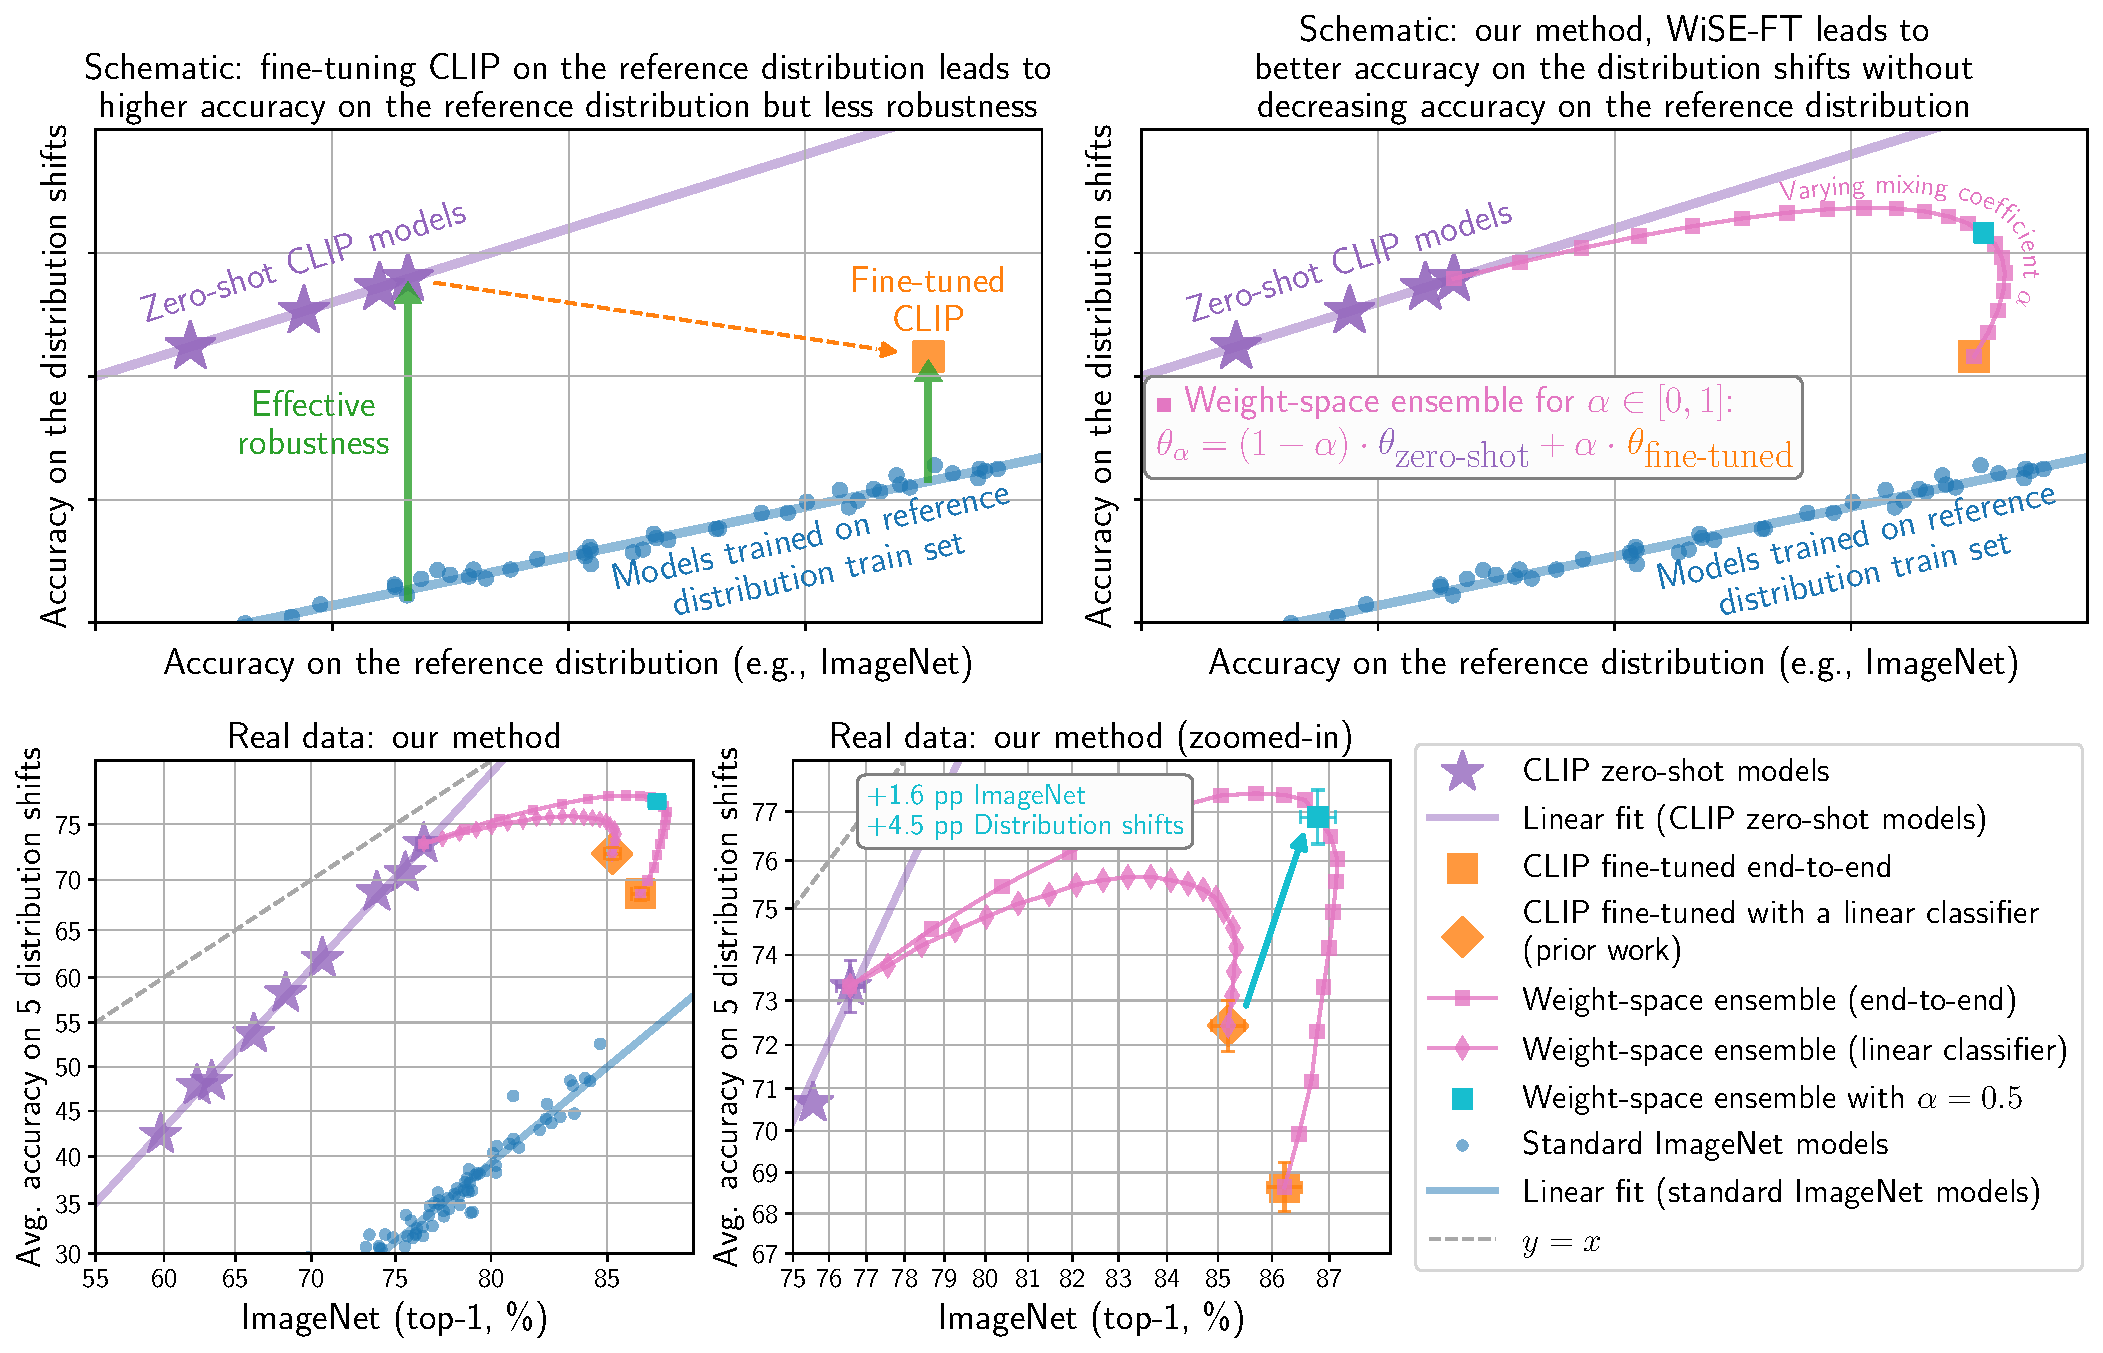
\includegraphics[width=\textwidth]{figures/fig1_new.pdf}
    \caption{
    \textbf{(Top left)} Zero-shot CLIP models exhibit moderate accuracy on the reference distribution ($x$-axis, the target for fine-tuning) and high effective robustness (accuracy on the distribution shifts beyond the baseline models).
    In contrast, standard fine-tuning---either end-to-end or with a linear classifier (final layer)---attains higher accuracy on the reference distribution but less effective robustness.
    \textbf{(Top right)} Our method linearly interpolates between the zero-shot and fine-tuned models with a mixing coefficient $\alpha \in [0,1]$. \textbf{(Bottom)} On five distribution shifts derived from ImageNet (ImageNetV2, ImageNet-R, ImageNet Sketch, ObjectNet, and ImageNet-A), WiSE-FT improves average accuracy relative to both the zero-shot and fine-tuned models while maintaining or improving accuracy on ImageNet.
    }
    \label{fig:fig1}
\end{figure*}


As pre-trained models are becoming a cornerstone of machine learning, techniques for fine-tuning them on downstream applications are increasingly important.
Indeed, the question of robustly fine-tuning pre-trained models has recently also been raised as an open problem by several authors 
\cite{andreassen2021evolution,bommasani2021opportunities,radford2021learning,pham2021scaling}.
\citet{andreassen2021evolution} explored several fine-tuning approaches but found that none yielded models with improved robustness at high accuracy.
Furthermore, \citet{taori2020measuring} demonstrated that no current algorithmic robustness interventions provide consistent gains across the distribution shifts where zero-shot models excel.


In this paper, we conduct an empirical investigation to understand and improve fine-tuning of zero-shot models from a distributional robustness perspective.
We begin by measuring how different fine-tuning approaches (last-layer vs.\ end-to-end fine-tuning, hyperparameter changes, etc.) affect the accuracy under distribution shift of the resulting fine-tuned models.
Our empirical analysis uncovers two key issues in the standard fine-tuning process.
First, the robustness of fine-tuned models varies substantially under even small changes in hyperparameters, but the best hyperparameters cannot be inferred from accuracy on the target distribution alone.
Second, more aggressive fine-tuning (e.g., using a larger learning rate) yields larger accuracy improvements on the target distribution, but can also reduce accuracy under distribution shift by a large amount.



Motivated by the above concerns, we propose a robust way of fine-tuning zero-shot models that addresses the aforementioned trade-off and achieves the best of both worlds: increased performance under distribution shift while maintaining or even improving accuracy on the target distribution relative to standard fine-tuning.
In addition, our method simplifies the choice of hyperparameters in the fine-tuning process.

Our method (Figure \ref{fig:fig1}) has two steps: first, we fine-tune the zero-shot model on the target distribution.
Second, we combine the original zero-shot and fine-tuned models by linearly interpolating between their weights, which we refer to as weight-space ensembling.
Interpolating model parameters is a classical idea in convex optimization dating back decades (e.g., see~\cite{ruppert1988efficient, polyak1990new}).
Here, we empirically study model interpolation for non-convex models from the perspective of distributional robustness.
Interestingly, linear interpolation in weight-space still succeeds despite the non-linearity in the activation functions of the neural networks.


Weight-space ensembles for fine-tuning (WiSE-FT) substantially improve accuracy under distribution shift compared to prior work while maintaining high performance on the target distribution.
Concretely, on ImageNet \cite{deng2009imagenet} and five of the natural distribution shifts studied by \citet{radford2021learning}, WiSE-FT applied to standard end-to-end fine-tuning improves accuracy under distribution shift by 4 to 6 percentage points (pp) over prior work while maintaining or improving the ImageNet accuracy of the fine-tuned CLIP model.
Relative to the zero-shot model, WiSE-FT improves accuracy under distribution shift by 1 to 9 pp.
Moreover, WiSE-FT improves over a range of alternative approaches such as regularization and evaluating at various points throughout fine-tuning.
These robustness gains come at no additional computational cost during fine-tuning or inference.

While our investigation centers around CLIP, we observe similar trends for other zero-shot models including ALIGN~\cite{jia2021scaling}, BASIC~\cite{pham2021scaling}, and a ViT model pre-trained on JFT~\cite{dosovitskiy2021an}.
For instance, WiSE-FT improves the ImageNet accuracy of a fine-tuned BASIC-L model by 0.4 pp, while improving average accuracy under distribution shift by 2 to 11 pp.


To understand the robustness gains of WiSE-FT, we first study WiSE-FT when fine-tuning a linear classifier (last layer) as it is more amenable to analysis. In this linear case, our procedure is equivalent to ensembling the outputs of two models, and experiments point towards the complementarity of model predictions as a key property.
For end-to-end fine-tuning, we connect our observations  to earlier work on the phenomenology of deep learning.
\citet{neyshabur2020being} found that end-to-end fine-tuning the same model twice yielded two different solutions that were connected via a linear path in weight-space along which error remains low, known as linear mode connectivity \cite{frankle2020linear}.
Our observations suggest a similar phenomenon along the path generated by WiSE-FT, but the exact shape of the loss landscape and connection between error on the target and shifted distributions are still open problems.


In addition to the aforementioned ImageNet distribution shifts, WiSE-FT consistently improves robustness on a diverse set of six additional distribution shifts including:
(i) geographic shifts in satellite imagery and wildlife recognition (WILDS-FMoW, WILDS-iWildCam) \cite{wilds2021, christie2018functional, beery2021iwildcam},
(ii) reproductions of the popular image classification dataset CIFAR-10 with a distribution shift (CIFAR-10.1 and CIFAR-10.2)  \cite{pmlr-v97-recht19a, lu2020harder}, and
(iii) datasets with distribution shift induced by temporal perturbations in videos (ImageNet-Vid-Robust and YTBB-Robust) \cite{vidrobust}.
Beyond the robustness perspective, WiSE-FT also improves accuracy compared to standard fine-tuning, reducing the relative error rate by 4-49\% on a range of seven datasets: ImageNet, CIFAR-10, CIFAR-100 \cite{krizhevsky2009learning}, Describable Textures \cite{dtd}, Food-101 \cite{food101}, SUN397 \cite{sun397}, and Stanford Cars \cite{cars}.
Even when fine-tuning data is scarce, reflecting many application scenarios, we find that WiSE-FT improves performance.

Overall, WiSE-FT is simple, universally applicable in the problems we studied, and can be implemented in a few lines of code. 
Hence we encourage its adoption for fine-tuning zero-shot models.



 \begin{figure*}[t]
    \centering
    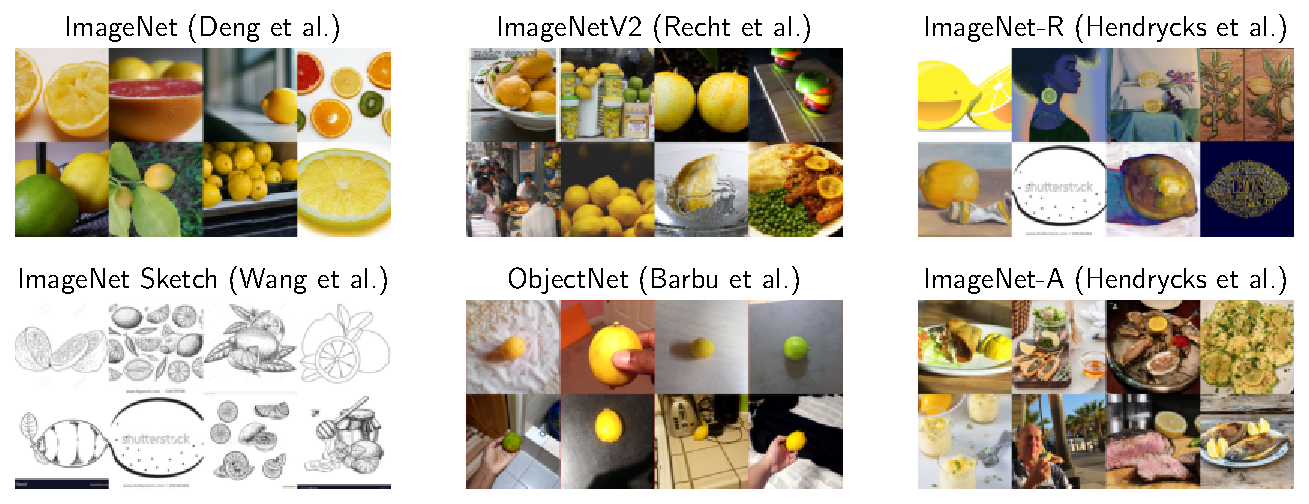
\includegraphics[width=0.9\textwidth]{figures/datasets_4cols.pdf}
    \caption{Samples of the class \textit{lemon}, from the reference distribution ImageNet \cite{deng2009imagenet} and the derived distribution shifts considered in our main experiments: ImageNet-V2 \cite{pmlr-v97-recht19a}, ImageNet-R \cite{imagenetr}, ImageNet Sketch \cite{imagenetsketch}, ObjectNet \cite{objectnet}, and ImageNet-A \cite{imageneta}.}
    \label{fig:data_samples}
\end{figure*}